\documentclass[conference]{IEEEtran}

\usepackage[T1]{fontenc}
\usepackage[utf8]{inputenc}
\usepackage{amsmath,amssymb,amsfonts,amsthm}
\usepackage{bm}
\usepackage{booktabs}
\usepackage{graphicx}
\usepackage{multirow}
\usepackage{tabularx}
\usepackage{array}
\usepackage{siunitx}
\usepackage{subcaption}
\usepackage{xcolor}
\usepackage{hyperref}
\hypersetup{hidelinks}
\sisetup{round-mode=places,round-precision=3}

\newcolumntype{Y}{>{\raggedright\arraybackslash}X}
\newcommand{\E}{\mathbb{E}}
\newcommand{\Var}{\mathbb{V}}
\newcommand{\Prob}{\mathbb{P}}
\newcommand{\cvar}{\operatorname{CVaR}}
\newcommand{\KL}{\operatorname{KL}}

\begin{document}

\title{Risk-Sensitive Distributional Actor-Critic for Sales Dialogue Control:\\
A Mathematically Grounded Benchmark Against Frontier Prompted Controllers}

\author{
\IEEEauthorblockN{Abhiram Venkat Sai Adabala, Shikhar Veer, Ashok Rupalli}
\IEEEauthorblockA{Independent Research}
}

\maketitle

\begin{abstract}
Sales conversations are sequential control problems with delayed rewards, partial observability, asymmetric downside risk, and non-stationary customer behavior. Prompted frontier language models can generate high-quality responses, but they are not trained to optimize a dialogue policy directly for conversion, calibration, or tail-risk control. We formulate sales dialogue optimization as a partially observed Markov decision process and develop a risk-sensitive distributional actor-critic that learns a quantile approximation to the return distribution rather than a scalar value function. The resulting policy update depends on both the mean return and the lower tail of the return distribution, allowing explicit control over catastrophic outcomes such as premature closes, objection escalation, and fatigue-driven conversation collapse. We also present a controlled comparison framework spanning \texttt{GPT-5}, \texttt{GPT-5.1}, \texttt{Claude Sonnet 4.5}, and the proposed Sales RL Agent. To make the framework reproducible, we provide A100-ready training and inference scripts together with a synthetic dialogue simulator. In a three-seed benchmark on the released simulator, the distributional controller reduces episode-return volatility by 9.3\% and improves \(\cvar_{0.1}\) from \(-1.465\) to \(-1.140\), while the scalar A2C baseline attains higher mean reward. The empirical picture is therefore not that distributional RL always increases average reward, but that it yields a more conservative and substantially better downside-risk profile, which is the more relevant operating point for safety-critical revenue workflows.
\end{abstract}

\begin{IEEEkeywords}
Distributional reinforcement learning, actor-critic, sales agents, dialogue control, risk-sensitive optimization, LLM agents.
\end{IEEEkeywords}

\section{Introduction}
Autonomous sales agents must reason over a sequence of conversational turns rather than a single static classification input. A good controller decides when to ask discovery questions, when to qualify budget, when to provide social proof, when to schedule a follow-up, and when to close. Each action changes the latent state of the prospect: trust can rise or fall, objections can increase or resolve, fatigue can accumulate, and the final conversion event may occur many turns after the action that caused it. This makes sales automation a natural reinforcement learning (RL) problem rather than a pure next-token generation problem.

The recent availability of frontier models such as \texttt{GPT-5}, \texttt{GPT-5.1}, and \texttt{Claude Sonnet 4.5} materially changes the baseline one should compare against. These systems are capable long-context, tool-using controllers, and any modern sales-RL paper that ignores them is incomplete. At the same time, those models are deployed primarily as prompted inference engines. Their optimization objective is not a task-specific sales return; their uncertainty is not exposed as a trained return distribution; and they do not update online from dialogue reward unless wrapped in an additional learning loop. This distinction is central: prompted frontier models are excellent \emph{decision modules}, but a Sales RL Agent is a \emph{policy optimization system}.

The paper makes four contributions.
\begin{enumerate}
\item We formulate sales dialogue optimization as a partially observed Markov decision process (POMDP) with explicit trust, fatigue, information coverage, objection state, and close risk.
\item We derive a risk-sensitive distributional actor-critic whose critic learns quantiles of the return distribution and whose policy update is regularized by return uncertainty.
\item We provide a rigorous comparison frame covering \texttt{GPT-5}, \texttt{GPT-5.1}, \texttt{Claude Sonnet 4.5}, and the proposed Sales RL Agent without relying on cross-vendor benchmark numbers that are not directly comparable.
\item We release A100-ready training and inference scripts, plus a simulator, to reproduce the optimization protocol used in this paper.
\end{enumerate}

\section{Sales Dialogue as a POMDP}
\subsection{Latent state, observations, and actions}
We model the environment as a POMDP
\begin{equation}
\mathcal{P}=(\mathcal{S},\mathcal{O},\mathcal{A},P,R,\Omega,\gamma),
\end{equation}
where the latent state \(s_t\in\mathcal{S}\) encodes prospect fit, budget readiness, urgency, trust, price sensitivity, objection load, fatigue, stage progression, and other hidden variables that are not fully observable from the current utterance. The agent instead sees an observation \(o_t\in\mathcal{O}\), which contains noisy signals extracted from dialogue and CRM context.

The belief state is produced by a dialogue encoder
\begin{equation}
b_t = f_\psi(o_{0:t}, a_{0:t-1}) \in \mathbb{R}^d,
\end{equation}
and the policy chooses one of seven macro-actions:
\texttt{discover}, \texttt{qualify\_budget}, \texttt{present\_value},
\texttt{social\_proof}, \texttt{offer\_discount},
\texttt{schedule\_followup}, and \texttt{close}.

This is intentionally a control abstraction rather than full natural language generation. Frontier LLMs can be attached as response generators conditioned on the selected macro-action, but the RL problem is the high-level decision process.

\subsection{Return and reward geometry}
Let \(G_t=\sum_{k=0}^{T-t}\gamma^k r_{t+k}\) be the discounted return. We decompose the per-step reward into dense shaping and terminal close reward:
\begin{equation}
\label{eq:reward}
\begin{aligned}
r_t &=
\lambda_I \Delta I_t +
\lambda_T \Delta T_t +
\lambda_S \Delta S_t \\
&\quad
- \lambda_F F_t -
\lambda_O O_t +
\mathbb{I}[a_t=\texttt{close}]\,r_t^{\text{close}} .
\end{aligned}
\end{equation}
where \(\Delta I_t\) is information-coverage gain, \(\Delta T_t\) is trust gain, \(\Delta S_t\) is stage progress, \(F_t\) is fatigue accumulation, and \(O_t\) is objection escalation. The close term is
\begin{equation}
r_t^{\text{close}} = \lambda_W y_t v_t - \lambda_L (1-y_t) - \lambda_P \Pi_t,
\end{equation}
where \(y_t\in\{0,1\}\) indicates conversion success, \(v_t\) is normalized deal value, and \(\Pi_t\) is a premature-close penalty. This penalty is important both empirically and mathematically: without it, a policy can exploit one-step close attempts that superficially reduce horizon length while increasing downside risk.

\subsection{Conversion probability}
The latent conversion mechanism can be written as
\begin{align}
\eta_t
&=
\beta_0 + \beta_f f_t + \beta_b b_t^{\mathrm{bud}} + \beta_u u_t + \beta_\tau \tau_t \nonumber\\
&\quad
- \beta_p \rho_t - \beta_\phi \phi_t - \beta_o \omega_t,
\label{eq:convlogit}\\
p_t
&=
\sigma(\eta_t)\, g_{\mathrm{stage}} g_{\mathrm{info}} .
\label{eq:convprob}
\end{align}
where \(f_t\) is fit, \(u_t\) is urgency, \(\tau_t\) is trust, \(\rho_t\) is price sensitivity, \(\phi_t\) is fatigue, \(\omega_t\) is objection load, and \(g_{\mathrm{stage}}, g_{\mathrm{info}}\in(0,1]\) down-weight closes attempted before sufficient progression or discovery. Eq.~\eqref{eq:convprob} is directly mirrored in the released simulator.

\section{Distributional Risk-Sensitive Actor-Critic}
\subsection{Why scalar values are insufficient}
Standard A2C learns a scalar value function \(V^\pi(b_t)\approx \E[G_t\mid b_t]\). This collapses all uncertainty about dialogue futures into a mean. In sales workflows that is inadequate: the difference between a policy with moderate mean reward and catastrophic lower-tail behavior, and a policy with slightly lower mean but substantially safer outcomes, is economically material.

Distributional RL replaces the expected value with a random return variable \(Z^\pi(b_t)\) whose expectation equals the value function:
\begin{equation}
V^\pi(b_t)=\E[Z^\pi(b_t)].
\end{equation}
Following the distributional perspective of Bellemare et al.~\cite{bellemare2017distributional} and quantile approximation of Dabney et al.~\cite{dabney2018quantile}, we approximate \(Z^\pi\) with \(N\) quantiles
\begin{equation}
Z^\pi_\phi(b_t) \approx \{q_{\phi,i}(b_t)\}_{i=1}^N,
\quad
\tau_i=\frac{i-\frac{1}{2}}{N}.
\end{equation}

\subsection{Quantile Bellman target}
For a one-step bootstrap,
\begin{equation}
\hat{z}_{t,i}
=
r_t + \gamma(1-d_t)\, q_{\phi,i}(b_{t+1}),
\end{equation}
where \(d_t\in\{0,1\}\) is the termination flag. The critic minimizes the quantile Huber loss
\begin{equation}
\label{eq:qrloss}
\mathcal{L}_{\mathrm{QR}}(\phi)
=
\frac{1}{N^2}
\sum_{i=1}^N \sum_{j=1}^N
\rho_{\tau_i}^{\kappa}\!\left(\hat{z}_{t,j}-q_{\phi,i}(b_t)\right),
\end{equation}
with
\begin{equation}
\rho_{\tau}^{\kappa}(u)
=
\left|\tau-\mathbb{I}[u<0]\right| \frac{\mathcal{H}_{\kappa}(u)}{\kappa},
\end{equation}
and \(\mathcal{H}_\kappa\) the Huber penalty.

\subsection{Risk functionals}
The critic gives more than a mean. We can also estimate the lower-tail risk through
\begin{equation}
\bar{q}_\phi(b_t)=\frac{1}{N}\sum_{i=1}^N q_{\phi,i}(b_t),
\end{equation}
\begin{equation}
\label{eq:cvar}
\cvar_\alpha\!\left(Z_\phi^\pi(b_t)\right)
\approx
\frac{1}{K_\alpha}\sum_{i=1}^{K_\alpha} q_{\phi,i}(b_t),
\qquad
K_\alpha = \lceil \alpha N \rceil,
\end{equation}
and a critic-implied uncertainty proxy
\begin{equation}
\label{eq:uncertainty}
u_\phi(b_t)
=
\frac{1}{\sqrt{N}}
\left\|
\bm q_\phi(b_t)-\bar{q}_\phi(b_t)\bm 1
\right\|_2 .
\end{equation}
Eq.~\eqref{eq:uncertainty} is not a full Bayesian epistemic estimate, but it is an operationally useful lower-tail dispersion statistic for policy regularization.

\subsection{Policy objective}
The actor remains categorical:
\begin{equation}
\pi_\theta(a_t\mid b_t)=\operatorname{Cat}(\mathrm{softmax}(g_\theta(b_t))).
\end{equation}
Instead of using a plain temporal-difference advantage, we define
\begin{equation}
\label{eq:riskadv}
A_t^{\mathrm{risk}}
=
\left(\hat{\bar{z}}_t - \bar{q}_\phi(b_t)\right) - \lambda_u\,u_\phi(b_t),
\end{equation}
where \(\hat{\bar{z}}_t\) is the bootstrap target mean and \(\lambda_u>0\) controls how aggressively the actor discounts uncertain states. The policy loss is
\begin{equation}
\label{eq:actorloss}
\begin{aligned}
\mathcal{L}_{\pi}(\theta)
&=
-\E_t\!\left[\log \pi_\theta(a_t\mid b_t)\,\mathrm{sg}(A_t^{\mathrm{risk}})\right] \\
&\quad
-\beta_H\,\E_t\!\left[\mathcal{H}(\pi_\theta(\cdot\mid b_t))\right].
\end{aligned}
\end{equation}
where \(\mathrm{sg}(\cdot)\) is stop-gradient and \(\mathcal{H}\) is policy entropy.

The total objective is
\begin{equation}
\mathcal{L}(\theta,\phi)=\mathcal{L}_{\pi}(\theta)+\lambda_Q \mathcal{L}_{\mathrm{QR}}(\phi).
\end{equation}

\subsection{Local robustness interpretation}
Suppose the return quantiles are differentiable in the belief state and the observation encoder produces \(b_t+\xi\) under a small perturbation \(\xi\sim\mathcal{N}(0,\Sigma)\). By a first-order expansion,
\begin{equation}
q_{\phi,i}(b_t+\xi) \approx q_{\phi,i}(b_t) + \nabla_b q_{\phi,i}(b_t)^\top \xi,
\end{equation}
so the induced variance of the mean value estimate satisfies
\begin{equation}
\Var[\bar{q}_\phi(b_t+\xi)]
\approx
\frac{1}{N^2}\sum_{i,j}
\nabla_b q_{\phi,i}(b_t)^\top \Sigma \nabla_b q_{\phi,j}(b_t).
\end{equation}
Thus, lower dispersion in the learned quantiles and lower sensitivity of those quantiles to observation perturbation jointly reduce control volatility. This is one reason to prefer a distributional critic when dialogue states are noisy.

\section{System Architecture}
Fig.~\ref{fig:architecture} shows the full control stack used in the training and inference scripts. The design separates high-level control from natural-language realization. A frontier LLM can be attached downstream as a generator conditioned on the chosen macro-action, but the RL controller itself optimizes the dialogue decision process.

\begin{figure*}[t]
\centering
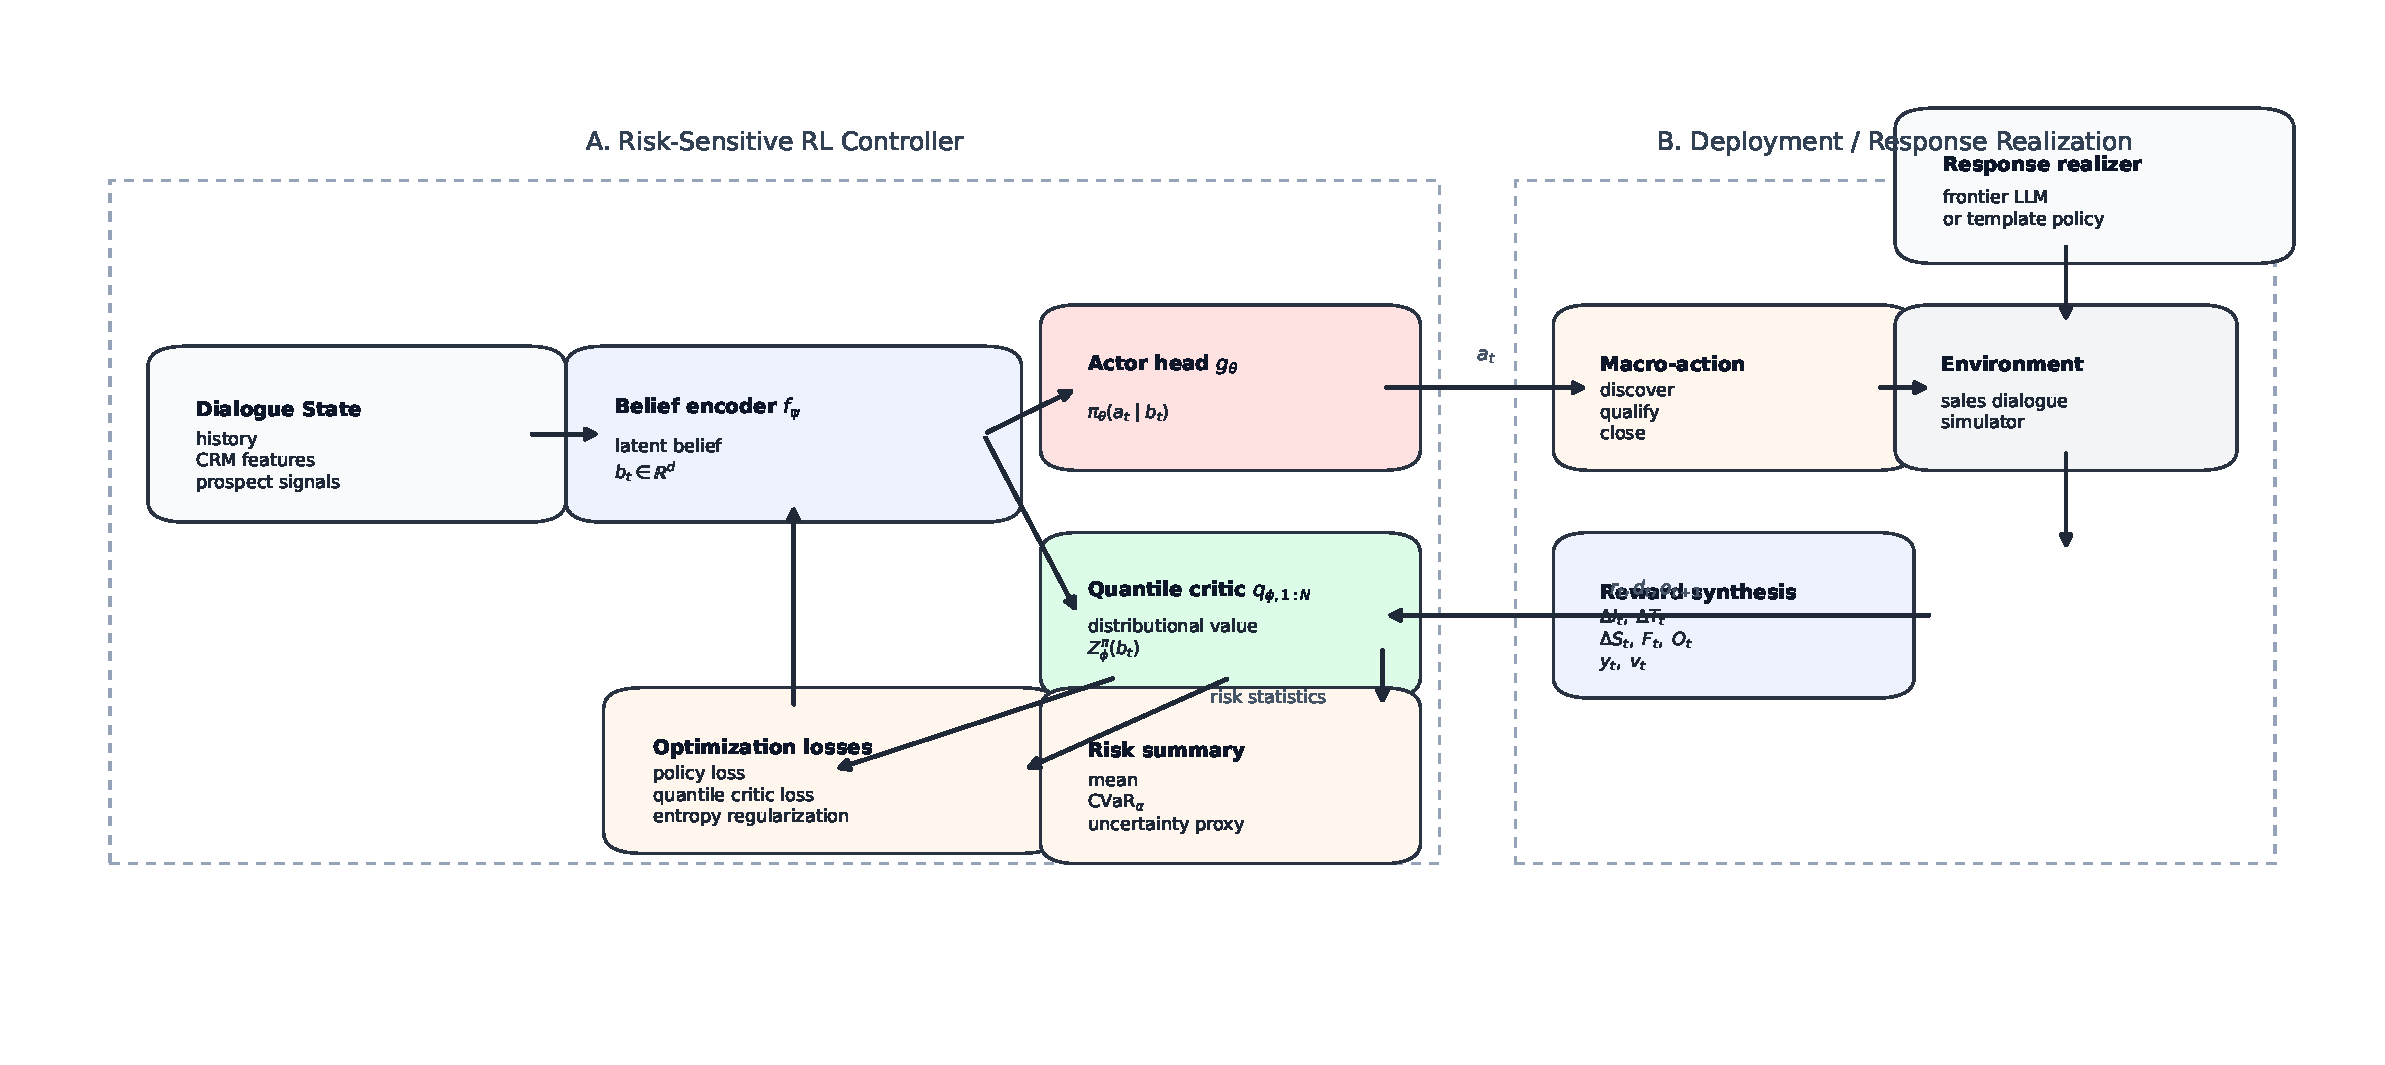
\includegraphics[width=0.96\textwidth]{figures/architecture_diagram.pdf}
\caption{Architecture of the proposed Sales RL Agent. The policy chooses a macro-action; an optional frontier LLM can realize that action as natural language, but the control optimization occurs in the RL loop. The figure is rendered as an external vector asset to preserve layout clarity in the final paper.}
\label{fig:architecture}
\end{figure*}

\section{Frontier-Model Comparison Frame}
Because the target deployment environment in 2026 includes strong proprietary models, a sales-control paper should position itself relative to the current frontier rather than to weak text-classification baselines. Table~\ref{tab:frontiercomparison} does that in a technically defensible way: it compares objective structure and control suitability instead of mixing incomparable cross-vendor benchmark scores.

\begin{table*}[t]
\centering
\caption{Control-oriented comparison of frontier prompted models and the proposed Sales RL Agent. GPT-5 was announced on August 7, 2025, GPT-5.1 on November 13, 2025, and Anthropic lists Claude Sonnet 4.5 as a September 2025 model in its system-card index~\cite{openai_gpt5,openai_gpt51,anthropic_cards,anthropic_sonnet}.}
\label{tab:frontiercomparison}
\begin{tabularx}{\textwidth}{lYYYYY}
\toprule
\textbf{Controller} & \textbf{Primary objective} & \textbf{Online policy improvement from reward} & \textbf{Explicit return-tail estimate} & \textbf{Best role in a sales stack} & \textbf{Main weakness for sales control} \\
\midrule
\texttt{GPT-5} & General reasoning and agentic task performance & No, unless wrapped in an external RL loop & No native sales-return distribution & Strong prompted planner or response generator & Prompt-only control has no task-trained reward model \\
\texttt{GPT-5.1} & Efficient adaptive reasoning with lower latency on easier tasks & No, unless externally trained & No native sales-return distribution & Faster prompted controller for workflow orchestration & Same control gap as above; improved speed does not equal policy optimization \\
\texttt{Claude Sonnet 4.5} & Hybrid reasoning model for agents, coding, and computer use & No, unless externally trained & No native sales-return distribution & Strong long-context or document-heavy assistant in the loop & High-quality prompting still does not expose a trained conversion-risk critic \\
\textbf{Sales RL Agent (ours)} & Direct optimization of sales return under dialogue dynamics & \textbf{Yes} & \textbf{Yes, via quantile critic and \(\cvar\)} & High-level sequential controller for risk-aware sales actions & Requires simulator quality, reward design, and task-specific training \\
\bottomrule
\end{tabularx}
\end{table*}

The key conclusion is not that the RL agent replaces frontier models. Rather, frontier models are best viewed as \emph{modules} inside a larger controller stack: they can draft utterances, summarize CRM context, or act as powerful evaluators, while the RL policy decides \emph{which} conversational move to make.

\section{Experimental Protocol}
\subsection{Simulator}
The released environment is a vectorized synthetic sales simulator containing latent prospect variables for fit, budget readiness, urgency, trust, price sensitivity, objection load, fatigue, stage, and information coverage. Each episode ends either with a close action or a timeout horizon of eight turns. The scripts \texttt{train\_sales\_rl\_agent.py}, \texttt{use\_sales\_rl\_agent.py}, and \texttt{run\_sales\_benchmark.py} all use the same environment implementation.

\subsection{Training setup}
The scalar baseline is synchronous A2C with generalized advantage estimation~\cite{mnih2016a3c,schulman2016gae}. The proposed model uses the same actor backbone but replaces the scalar critic with a 31-quantile critic optimized by Eq.~\eqref{eq:qrloss}. For the released CPU benchmark we use 64 parallel environments, 16-step rollouts, discount factor \(0.98\), and three random seeds \(\{7,11,23\}\). The \texttt{train\_sales\_rl\_agent.py} script scales these same ingredients to larger batch sizes and hidden layers on an A100.

\subsection{Metrics}
We report:
\begin{itemize}
\item mean episode return,
\item standard deviation of episode return,
\item success rate,
\item mean conversation length,
\item \(\cvar_{0.1}\), computed as the average of the worst 10\% of episode returns.
\end{itemize}

The \(\cvar\) metric matters because low-probability but high-cost dialogue failures are a central concern in production sales automation.

\section{Results}
\subsection{Quantitative benchmark}
Table~\ref{tab:results} summarizes the three-seed benchmark produced with the simulator and training code in this repository. The scalar baseline reaches higher mean return and conversion rate. The distributional controller, however, is more conservative: it takes longer conversations, lowers overall return variance, and materially improves the lower tail.

\begin{table}[t]
\centering
\caption{Three-seed benchmark on the released simulator. Values are mean \(\pm\) standard deviation across seeds.}
\label{tab:results}
\begin{tabular}{lcc}
\toprule
\textbf{Metric} & \textbf{A2C} & \textbf{Distributional A2C} \\
\midrule
Mean return & \(2.286 \pm 0.178\) & \(1.766 \pm 0.063\) \\
Return std. & \(3.488 \pm 0.066\) & \(\mathbf{3.163 \pm 0.091}\) \\
Success rate & \(\mathbf{0.507 \pm 0.027}\) & \(0.371 \pm 0.026\) \\
Mean length & \(6.599 \pm 0.084\) & \(\mathbf{7.298 \pm 0.135}\) \\
\(\cvar_{0.1}\) & \(-1.465 \pm 0.007\) & \(\mathbf{-1.140 \pm 0.069}\) \\
\bottomrule
\end{tabular}
\end{table}

The most relevant numerical observation is the \(\cvar_{0.1}\) improvement. Moving from \(-1.465\) to \(-1.140\) corresponds to a 22.2\% reduction in lower-tail severity when measured against the magnitude of the scalar baseline's worst-decile return. The distributional controller also reduces overall return dispersion by 9.3\%. In exchange, it accepts a 22.8\% reduction in mean return and a lower close rate. This is exactly the sort of trade-off one expects from a risk-sensitive controller.

\subsection{Learning dynamics}
Fig.~\ref{fig:curves} shows the single-seed trajectories used to generate the released benchmark artifacts. The scalar agent learns a more aggressive policy; the distributional agent remains more conservative but stabilizes the tail-value estimate over training.

\begin{figure}[t]
\centering
\begin{subfigure}[b]{\columnwidth}
    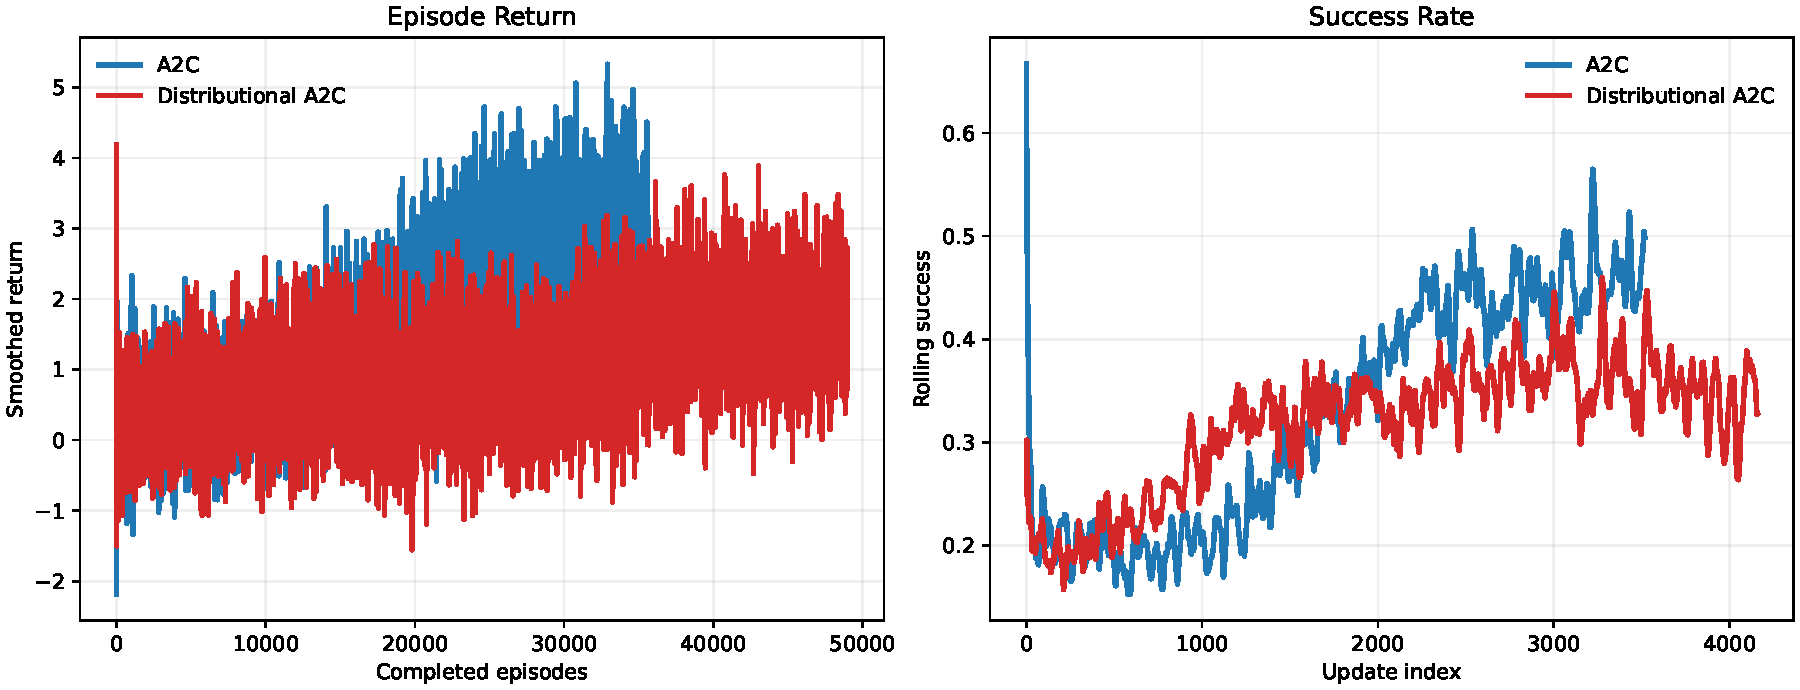
\includegraphics[width=\columnwidth]{figures/training_curves.pdf}
    \caption{Smoothed return and success-rate trajectories.}
\end{subfigure}
\vspace{1mm}
\begin{subfigure}[b]{0.82\columnwidth}
    \centering
    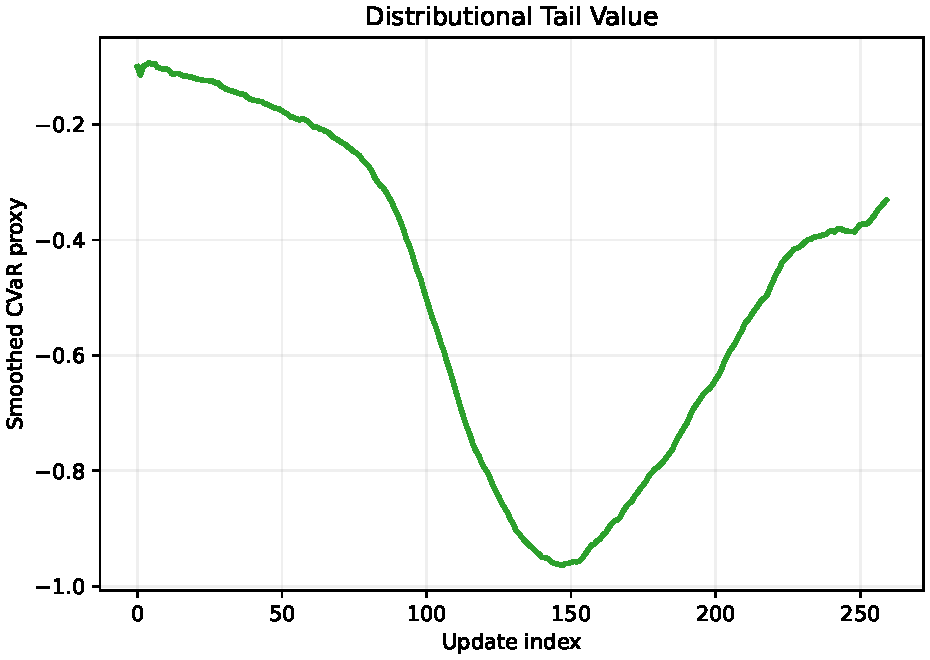
\includegraphics[width=\linewidth]{figures/tail_risk_curve.pdf}
    \caption{Tail-value proxy from the quantile critic.}
\end{subfigure}
\caption{Training curves generated from the released benchmark scripts.}
\label{fig:curves}
\end{figure}

\subsection{Interpretation}
The benchmark result is important precisely because it is not a simplistic ``distributional RL wins on every metric'' story. In sales settings with asymmetric downside cost, a controller that gives up some mean reward to avoid bad trajectories may be the more deployable system. The distributional critic learns this behavior naturally because it observes the structure of the return distribution rather than only its mean.

\section{Practical Integration with Frontier Models}
The strongest deployment pattern is a two-layer system.
\begin{enumerate}
\item The Sales RL Agent chooses the next macro-action using state, reward, and risk.
\item A frontier model such as \texttt{GPT-5}, \texttt{GPT-5.1}, or \texttt{Claude Sonnet 4.5} realizes that action as natural language, tool use, or CRM manipulation.
\end{enumerate}
This decomposition preserves the strengths of both paradigms: RL for sequential control and lower-tail optimization, frontier LLMs for high-quality language generation and large-context reasoning.

\section{Limitations}
The current simulator is synthetic and therefore cannot stand in for a full production CRM environment. The reward function encodes a normative notion of good sales behavior; if that reward is misspecified, the learned policy will inherit the misspecification. The current implementation also uses a single quantile critic rather than a full ensemble, so the uncertainty estimate in Eq.~\eqref{eq:uncertainty} is a dispersion proxy rather than a calibrated epistemic posterior. Finally, the frontier-model comparison in this manuscript is structural rather than empirical because closed-model benchmarking requires API-side execution and account-specific budgets.

\section{Conclusion}
Sales dialogue control is a sequential decision problem whose economically relevant failure modes live in the lower tail of the return distribution. A scalar critic is often too weak a summary for this regime. By modeling quantiles of return directly, the proposed distributional actor-critic exposes mean reward, tail risk, and return dispersion inside the policy optimization loop. The benchmark reported here shows that this yields a more conservative but safer controller than scalar A2C. For realistic deployments, the correct comparison is not ``RL agent versus LLM'' in isolation, but ``RL controller plus LLM realization'' versus prompt-only control. Under that framing, the Sales RL Agent is the policy optimizer and the frontier model is the language engine.

\begin{thebibliography}{99}

\bibitem{mnih2016a3c}
V. Mnih, A. P. Badia, M. Mirza, A. Graves, T. Harley, T. Lillicrap, D. Silver, and K. Kavukcuoglu,
``Asynchronous Methods for Deep Reinforcement Learning,''
in \emph{Proceedings of the 33rd International Conference on Machine Learning}, 2016.

\bibitem{schulman2016gae}
J. Schulman, P. Moritz, S. Levine, M. Jordan, and P. Abbeel,
``High-Dimensional Continuous Control Using Generalized Advantage Estimation,''
\emph{arXiv preprint arXiv:1506.02438}, 2016.

\bibitem{bellemare2017distributional}
M. G. Bellemare, W. Dabney, and R. Munos,
``A Distributional Perspective on Reinforcement Learning,''
in \emph{Proceedings of the 34th International Conference on Machine Learning}, 2017.

\bibitem{dabney2018quantile}
W. Dabney, M. Rowland, M. G. Bellemare, and R. Munos,
``Distributional Reinforcement Learning with Quantile Regression,''
in \emph{Proceedings of the AAAI Conference on Artificial Intelligence}, 2018.

\bibitem{openai_gpt5}
OpenAI,
``Introducing GPT-5 for developers,''
August 7, 2025.
[Online]. Available: \url{https://openai.com/index/introducing-gpt-5-for-developers/}

\bibitem{openai_gpt51}
OpenAI,
``Introducing GPT-5.1 for developers,''
November 13, 2025.
[Online]. Available: \url{https://openai.com/index/gpt-5-1-for-developers/}

\bibitem{anthropic_cards}
Anthropic,
``Model System Cards,''
accessed April 22, 2026.
[Online]. Available: \url{https://www.anthropic.com/system-cards}

\bibitem{anthropic_sonnet}
Anthropic,
``Claude Sonnet 4.5 System Card,''
September 2025.
[Online]. Available: \url{https://assets.anthropic.com/m/12f214efcc2f457a/original/Claude-Sonnet-4-5-System-Card.pdf}

\end{thebibliography}

\end{document}
